\documentclass[11pt,aspectratio=169]{beamer}
\usetheme{Marburg}
\graphicspath{{Arquivos/}}
\usepackage[utf8]{inputenc}
\setbeamertemplate{footline}[frame number]
\usepackage{cmbright}
\usepackage[T1]{fontenc}
\usepackage{amsmath}
\usepackage{amsfonts}
\usepackage{amssymb}
\usepackage{hyperref}
\usepackage{graphicx}
\author{Theodora Panagea - 1115201400135 \\ Anna-Aikaterini Kavvada - 1115201500050}
\newcommand{\TT}{From Linear to Conic Duality}
\newcommand{\TL}{Algorithmic Operational Research}
\newcommand{\DT}{Introduction}
\newcommand{\IN}{What is Conic Duality?}
\newcommand{\PI}{Conic Duality Theorem}
\newcommand{\PII}{Geometry of Primal and Dual Problems}
\newcommand{\PIII}{Applications of Conic Duality}
\newcommand{\PIV}{Is Something Wrong?}
\newcommand{\PV}{Consequences}
\newcommand{\BI}{Bibliography}

\title{\TT}
%\setbeamercovered{transparent} 
\setbeamertemplate{navigation symbols}{\href{https://github.com/AriannaK97/From-Linear-to-Conic-Duality}{Our Github Repository}}
\institute{Department of Informatics and Telecommunications \\ National and Kapodistrian University of Athens} 
\date{January 10, 2020} 
\begin{document}

\begin{frame}
\titlepage
\end{frame}

\LARGE

\section{\DT}
\begin{frame}{\TT}{\TL}
 \begin{block}{\DT}\pause
 \Large
\begin{center}\textbf{Linear Programming}\end{center}
$\bullet$ Specific computational techniques\\
$\bullet$ A number of general results, including those of (LP) \\
\hspace{4mm}Duality Theorem \\
 \end{block}
\end{frame}

\begin{frame}{\TT}{\TL}
 \begin{block}{\DT}
 \Large
\textbf{Linear Duality $\rightarrow$} one of the most important techniques of\\ \hspace{4cm} Linear Programming
\begin{center}\textbf{But...}\end{center}\textbf{Nonlinear cases $\rightarrow$} not applicable!\newline \newline
\textbf{\underline{Solution:}} Extension of (LP) techniques to (CP).
 \end{block}
\end{frame}

\begin{frame}{\TT}{\TL}
 \begin{block}{\DT}
 \Large
\textit{Generic (LP) Problem:}
$$\min\limits_{x}\{c^Tx | Ax \geq B \}$$
\textit{Generic (CP) Problem:}
$$\min\limits_{x}\{c^Tx | Ax \geq_\kappa b \},$$
where \textbf{K} is a regular cone (convex, pointed, closed and with a nonempty interior).
 \end{block}
\end{frame}

\section{\IN}
\begin{frame}{\TT}{\TL}
 \begin{block}{\IN}\pause
 \Large
\textbf{(LP):}
The need to get to a lower bound on the optimal value\\ \hspace{9mm} $c^*$, where 
$$c^* = \min\limits_{x}\{c^Tx | Ax \geq b \},$$
with constraint
$$\langle \lambda,A \rangle \equiv \lambda^T Ax \geq \lambda^T b \quad(Cons(\lambda))$$
and weight vectors 
$$\lambda \geq 0$$
 \end{block}
\end{frame}

\begin{frame}{\TT}{\TL}
 \begin{block}{\IN}
 \Large
 \textbf{(LP) Dual:}
$$\max\{b^T\lambda |\lambda \geq 0, A^T\lambda = c \},$$
\textit{After all, it is nothing but finding the best lower bound one can get in this fashion.}
 \end{block}
\end{frame}

\begin{frame}{\TT}{\TL}
 \begin{block}{\IN}
 \Large 
 \textbf{(CP):}
 Following the same scheme of LP, with the following\\ \hspace{9mm} primal
 $$\min\{c^Tx|Ax \geq_\kappa b \}$$\newline
 \textit{(?)What are the "admissible" weight vectors
 $$\langle \lambda, Ax \rangle \geq \langle \lambda,b \rangle$$ is a consequence of the vector inequality $Ax 
 \geq_{\kappa}b$?}
 \end{block}
\end{frame}

\begin{frame}{\TT}{\TL}
 \begin{block}{\IN}
\Large
 \textit{(?)What are the "admissible" weight vectors
 $$\langle \lambda, Ax \rangle \geq \langle \lambda,b \rangle$$ is a consequence of the vector inequality $Ax 
 \geq_{\kappa}b$?}\newline
 \underline{\textit{Answer:}}
 The same as to say what are the weight vectors $\lambda$\\ \hspace{19mm} such that 
 $$\forall \alpha \geq_{\kappa}0 : \quad \langle \lambda, \alpha \rangle \geq 0$$
 \end{block}
\end{frame}

\begin{frame}{\TT}{\TL}
 \begin{block}{\IN}
 \Large
 \underline{\textit{Observation:}} \newline When: \newline
 $\bullet \quad x$ is a feasible solution to (CP) \newline
 $\bullet \quad \lambda$ is an admissible weight vector, i.e., $\lambda \in K^*$\\ \hspace{7mm} where $K^*$ is dual cone of $K$\newline
 Then:
 $$(A^* \lambda)^T x \equiv \langle \lambda , Ax \rangle \geq \langle \lambda, b \rangle$$
 \end{block}
\end{frame}

\begin{frame}{\TT}{\TL}
 \begin{block}{\IN}
 \Large 
 For $(A^* \lambda)^T x \equiv \langle \lambda , Ax \rangle \geq \langle \lambda, b \rangle$, we need:\newline \newline
 $\bullet \quad A^* \lambda = c$\newline
 $\bullet \quad c^T x = (A^* \lambda)^T x = \langle \lambda,Ax\rangle \geq \langle b, \lambda \rangle$\newline \newline
 $\Rightarrow \hspace{1mm} \langle b, \lambda \rangle$: Lower bound on the optimal value of 
 (CP).\\
 \end{block}
\end{frame}

\begin{frame}{\TT}{\TL}
 \begin{block}{\IN}
 \Large
 \textbf{(CP) Dual:}
 \textit{The best bound is the optimal value in the problem:}
 $$\max\{\langle b, \lambda \rangle | A^*\lambda = c, \lambda \geq_{\kappa^*} 0 \}$$\newline
 \textit{which is the (CP) dual.}
 \end{block}
\end{frame}

\section{\PI}
\begin{frame}{\TT}{\TL}
 \begin{block}{\PI}\pause
 \Large
To establish Conic Duality (CD), we need:\newline \newline
$\bullet$ Proof of symmetry\\
$\bullet$ Weak Duality \\
$\bullet$ Regular Duality \\
$\bullet$ Strong Duality \\
 \end{block}
\end{frame}

\begin{frame}{\TT}{\TL}
 \begin{block}{\PI}
\Large
$\bullet$ Proof of Symmetry \newline \\
\hspace{3mm}
(P)\hspace{1mm} $\min\{c^Tx|Ax \geq_\kappa b \}$ \\
\hspace{3mm}
(D) $\max\{\langle b, \lambda \rangle | A^*\lambda = c, \lambda \geq_{\kappa^*} 0 \}$ \newline \\
\hspace{3mm} The (D) can be reformed as:\\ \hspace{13mm} (D') $\min\{-\langle b, \lambda \rangle | A^*\lambda = c, \lambda \geq_{\kappa^*} 0 \}$ \newline \\
\hspace{4mm} It's trivial that the dual of the (D') $\Rightarrow$ (P) \\
 \end{block}
\end{frame}

\begin{frame}{\TT}{\TL}
 \begin{block}{\PI}
\Large
$\bullet$ Weak Duality \newline \\
\begin{Theorem} If (D) feasible, and if (P) subfeasible, then the subvalue of (P) is upper-bounded by the value of (D). \newline
If (P) and (D) feasible, then the value of (P) is upper-bounded by the value of (D), and both are finite.
\end{Theorem}
 \end{block}
\end{frame}

\begin{frame}{\TT}{\TL}
 \begin{block}{\PI}
\Large
$\bullet$ Regular Duality \newline \\
\begin{Theorem} The (D) is feasible and has finite value $\beta$ if and only if the (P) is subfeasible and has finite subvalue $\gamma$. Also, $\beta = \gamma$. \newline \\

\end{Theorem}
The proof consists of applications of the Farkas lemma.
 \end{block}
\end{frame}

\begin{frame}{\TT}{\TL}
 \begin{block}{\PI}
\Large 
\vspace{3mm}
\textbf{The Farkas Lemma} \\
\begin{Lemma} Let $K \subseteq V$ be a closed convex cone, and $b \in W$. The system $Ax = b, x \in K$ is subfeasible if and only if every $y \in W$ with $A^Ty \in K^{\**}$ also satisfies $\langle y, b \rangle \geq 0$ \newline \\
 \newline \\

\end{Lemma}

 \end{block}
\end{frame}


\begin{frame}{\TT}{\TL}
 \begin{block}{\PI}
\Large
$\bullet$ Strong Duality \newline \\
\begin{Theorem} If (P) is feasible, has finite value $\gamma$ and has interior point $\Tilde{x}$, then (D) is feasible and has finite value $\beta = \gamma$. \newline \\

\end{Theorem}
The proof uses the Slater's constraint qualification.
 \end{block}
\end{frame}

\section{\PII}
\begin{frame}{\TT}{\TL}
 \begin{block}{\PII}\pause 
 \Large
(P)\hspace{1mm} $\min\{c^Tx|Ax \geq_\kappa b \}$\newline
\newline
(D) $\max\{\langle b, \lambda \rangle | A^*\lambda = c, \lambda \geq_{\kappa^*} 0 \}$\newline \\
\textbf{At first}, they look completely different...
 \end{block}
\end{frame}

\begin{frame}{\TT}{\TL}
 \begin{block}{\PII}
\Large
\newline
\begin{center}
    \textbf{But...}
\end{center}
The difference is just in data representation $\rightarrow$ Geometrically similar! 
 \end{block}
\end{frame}

\begin{frame}{\TT}{\TL}
 \begin{block}{\PII}
\Large
\textbf{In (D):} \newline
\hspace{2mm}$\bullet \quad max \langle b, \lambda \rangle$ \\
\hspace{2mm}$\bullet \quad L_{*} = \{ \lambda : A^* \lambda = c \}$: affine plane \\
\hspace{2mm}$\bullet \quad K_{*}$: cone \\
%----------------
\textbf{In (P):} \\
\hspace{2mm}$\bullet \quad y = Ax - b$: image of "true design" variables $x$ \\
\hspace{2mm}$\bullet \quad x \in R^n$ \\
\hspace{2mm}$\bullet \quad y \in L = \{ y = Ax - b: x \in R^n \}$: affine \\
\hspace{2mm}$\bullet \quad$\emph{iff} $x \in R^n \rightarrow$ feasible $\Rightarrow y \in K$ \\
 \end{block}
\end{frame}

\begin{frame}{\TT}{\TL}
 \begin{block}{\PII}
\Large
\newline
\vspace{2mm}
    \textbf{The objective:}
$$c^Tx = \langle d, Ax - b \rangle + \text{const} \equiv c \in \text{Im}{A^*}$$
where: \\
\hspace{2mm} $\bullet \quad (P) \text{ equals: }\min\limits_{y}\{ \langle d,y \rangle : y \in L, y \geq_{\kappa} 0 \}$ \\
\hspace{2mm} $\bullet \quad L = \text{Im}A - b$ \\
\hspace{2mm} $\bullet \quad A^*d = c, \hspace{4mm} d: \text{any vector}$
 \end{block}
\end{frame}

\begin{frame}{\TT}{\TL}
 \begin{block}{\PII}
\Large
\newline
\vspace{2mm}
    \textbf{Thus... } \newline \\
The primal problem, geometrically, is the problem of minimizing a linear form over the intersection of the affine plane $L$ with the cone $K$. \newline \\
The dual problem, similarly, is to maximize another linear form over the intersection of the affine plane $L_{\**}$ with the dual cone $K_{\**}$.
 \end{block}
\end{frame}

\begin{frame}{\TT}{\TL}
 \begin{block}{\PII}
\Large
\newline
\vspace{2mm}
   If conditions for (P) are not satisfied, the problem is: \newline \\
  \hspace{2mm} $\bullet$ unbounded below, or \\
  \hspace{2mm} $\bullet$ infeasible \\ \vspace{3mm}
  \hspace{2mm} $\Rightarrow$ We reject (P) from the very beginning. \\
 \end{block}
\end{frame}

\begin{frame}{\TT}{\TL}
 \begin{block}{\PII}
\Large
\newline
\begin{figure}
\begin{center}
  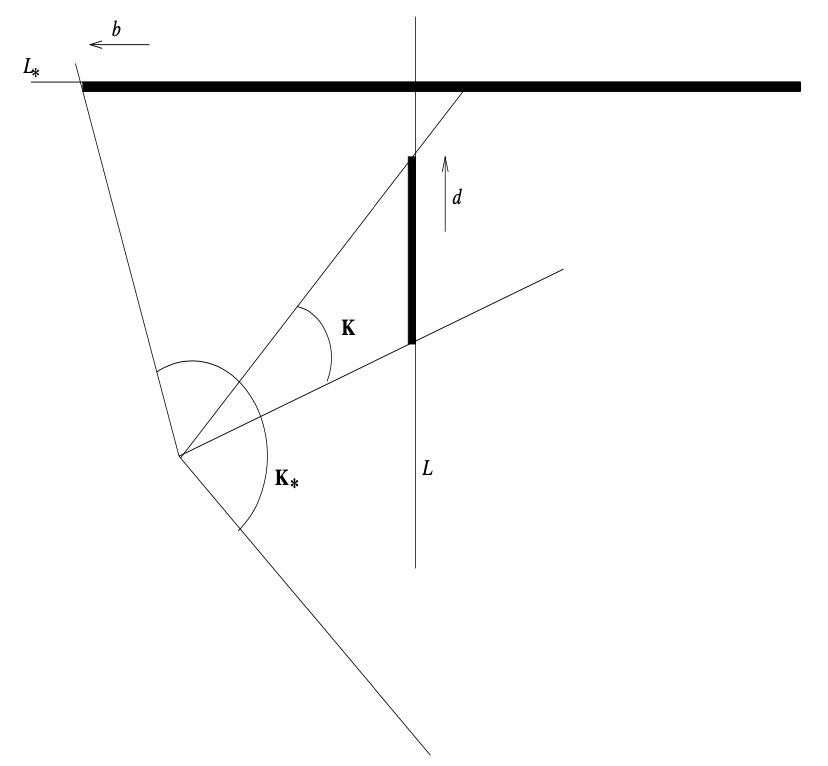
\includegraphics[scale = 0.3]{fig1.png}
 
  \caption{Primal-dual pair of conic problems \newline [bold: primal (vertical segment) and dual (horizontal ray) feasible sets]}
 \end{center}
\end{figure}
 \end{block}
\end{frame}

\begin{frame}{\TT}{\TL}
 \begin{block}{\PII}
\Large
\newline
\vspace{2mm}
  \hspace{2mm} $\bullet \quad K_{\**}$ dual of $K$ \\
  \hspace{2mm} $\bullet \quad L\perp L_{\**}$ \newline \\
  NOTE: The duality is completely symmetric (Weak Conic Duality Theorem) \\ \vspace{2mm}
 \hspace{2mm} $\Rightarrow \quad (K_{\**})_{\**} = K$ \\
 \hspace{2mm} $\Rightarrow \quad (L^{\perp})^{\perp} = L$
 \end{block}
\end{frame}

\section{\PIII}
\begin{frame}{\TT}{\TL}
 \begin{block}{So...}
\Large
\vspace{7.5mm}
\begin{figure}
\begin{center}
  
\includegraphics[scale = 0.2]{maths.jpg}
 \end{center}
\end{figure}
 \end{block}
\end{frame}

\begin{frame}{\TT}{\TL}
 \begin{block}{So...}
\Large
\textit{(?!)Where can all these maths, actually be applied?!} 
\begin{figure}
\begin{center}
  
\includegraphics[scale = 0.2]{maths.jpg}
 \end{center}
\end{figure}
 \end{block}
\end{frame}

\begin{frame}{\TT}{\TL}
 \begin{block}{\PIII}\pause
\Large
\hspace{2mm} $\bullet$ Self-Dual Cones \\
\hspace{2mm} $\bullet$ Second Order Cone Programming (SOCP) \\
\hspace{2mm} $\bullet$ Semidefinite Programming (SDP) \\
\hspace{2mm} $\bullet$ Distributionally Robust Learning (DRL) \\
 \end{block}
\end{frame}

\begin{frame}{\TT}{\TL}
 \begin{block}{\PIII}
\Large
More specifically, DRL is necessary for Machine Learning systems: When applied in the real world, performance may be significantly degraded, because of different distribution between test and training data. \\ DRL considers the worst-case distribution, minimizing the reweighted training loss and creating classifiers.
 \end{block}
\end{frame}

\section{\PIV}
\begin{frame}{\TT}{\TL}
 \begin{block}{\PIV}\pause
\Large
\textit{Well...}\newline \\
CP duality Theorem $\rightarrow$ weaker than LP duality Theorem
 \end{block}
\end{frame}

\section{\PIV}
\begin{frame}{\TT}{\TL}
 \begin{block}{\PIV}
\Large
\textbf{LP:}\\
$\bullet$ Feasibility (even non-strict) and boundedness of either\\
\hspace{4mm}primal or dual $\Rightarrow$ solvability of (P) and (D) equality\\
\hspace{4mm}between their optimal values\\
\textbf{CP:}\\
$\bullet$ If one of (P), (D) is essentially strictly feasible and\\
\hspace{4mm}bounded, then the other is solvable and $Opt(P) = Opt(D)$\\
$\bullet$ If both are essentially strictly feasible, then both are\\ 
\hspace{4mm}solvable, with $Opt(P) = Opt(D)$

 \end{block}
\end{frame}


\section{\PV}
\begin{frame}{\TT}{\TL}
 \begin{block}{\PV}\pause
\Large
$\bullet$ Sufficient condition for infeasibility \\
$\bullet$ The linear inequality of scalar $(S)$ is a consequence of a \\ 
\hspace{4mm} feasible system of linear inequalities $Ax \geq b$ \textit{iff} $(S)$ can be \\ 
\hspace{4mm} obtained from linear vector $(V)$ and the trivial 1 \geq 0 \\
$\bullet$  Robustness: are the properties for the (P) (feasibility, 
\\ \hspace{4mm} solvability, etc), stable with respect to perturbations of \\ 
\hspace{4mm} the data  (inexact data, adding noise during data 
\\ 
\hspace{4mm} processing) 
 \end{block}
\end{frame}

\section{\BI}
\begin{frame}{\TT}{\TL}
 \begin{block}{\BI}\pause
\Large
$[1]$ Ben-Tal, A. and Nemirovskiĭ, A. Lectures on Modern Convex Optimization. pp.52-71. (2013). \\
$[2]$ O.Güler. Foundations of Optimization. Graduate Texts in Mathematics. Springer New York, (2010). \\
$[3]$ David Williamson. Orie6300: Mathematical programming I, lecture 26. http://people.orie.cornell.edu/dpw/orie6300/Lectures/\\
lec26.pdf. \\

 \end{block}
\end{frame}

\begin{frame}{\TT}{\TL}
 \begin{block}{\BI}
\Large
$[4]$ B. Gartner and Matousek J. Approximation algorithms and semidefinite programming: Cone programming. http://www.ti.inf.ethz.ch/ew/lehre/ApproxSDP09/notes/\\conelp.pdf. \\
$[5]$ Weihua Hu et. al, Does Distributionally Robust Supervised Learning Give Robust Classifiers? (2018) arXiv:1611.02041v6 \\
$[6]$ Yinyu Ye. Conic Duality Theorems and Applications. Department of Management Science and Engineering, Stanford University. Chapters 4.1-4.2 and 6.1-6.4 . 
 \end{block}
\end{frame}

\begin{frame}{\TT}{\TL}
 \begin{block}{Thank you, next}
\Large
\begin{figure}
\begin{center}
  
\includegraphics[width = 8cm]{grand.jpg}
 \end{center}
\end{figure}
 \end{block}
\end{frame}


\end{document}